\subsection{Karten Finden}
\label{sec:kartenFinden}

Das folgende Verfahren soll in der Lage sein, in einem Videobild die gezeigten Karten zu finden.
Hierbei wird sich darauf beschränkt, dass Karten, die teilweise überdeckt sind, nicht gefunden werden.
Das Bild wird in einem Vorverarbeitungsschritt so bearbeitet, dass die Ränder der Karten klar abgehoben erkennbar sind. Auf diesem Bild wird dann nach Konturen gesucht, die denen einer Karte entsprechen.

Die Videobilder sind Farbbilder mit einer Auflösung von $1920 \times 1080$ Pixeln.
Das Verfahren wird anhand des Bildes in Abbildung \ref{fig:findCardsSample} veranschaulicht.

\begin{figure}[h]
    \centering
		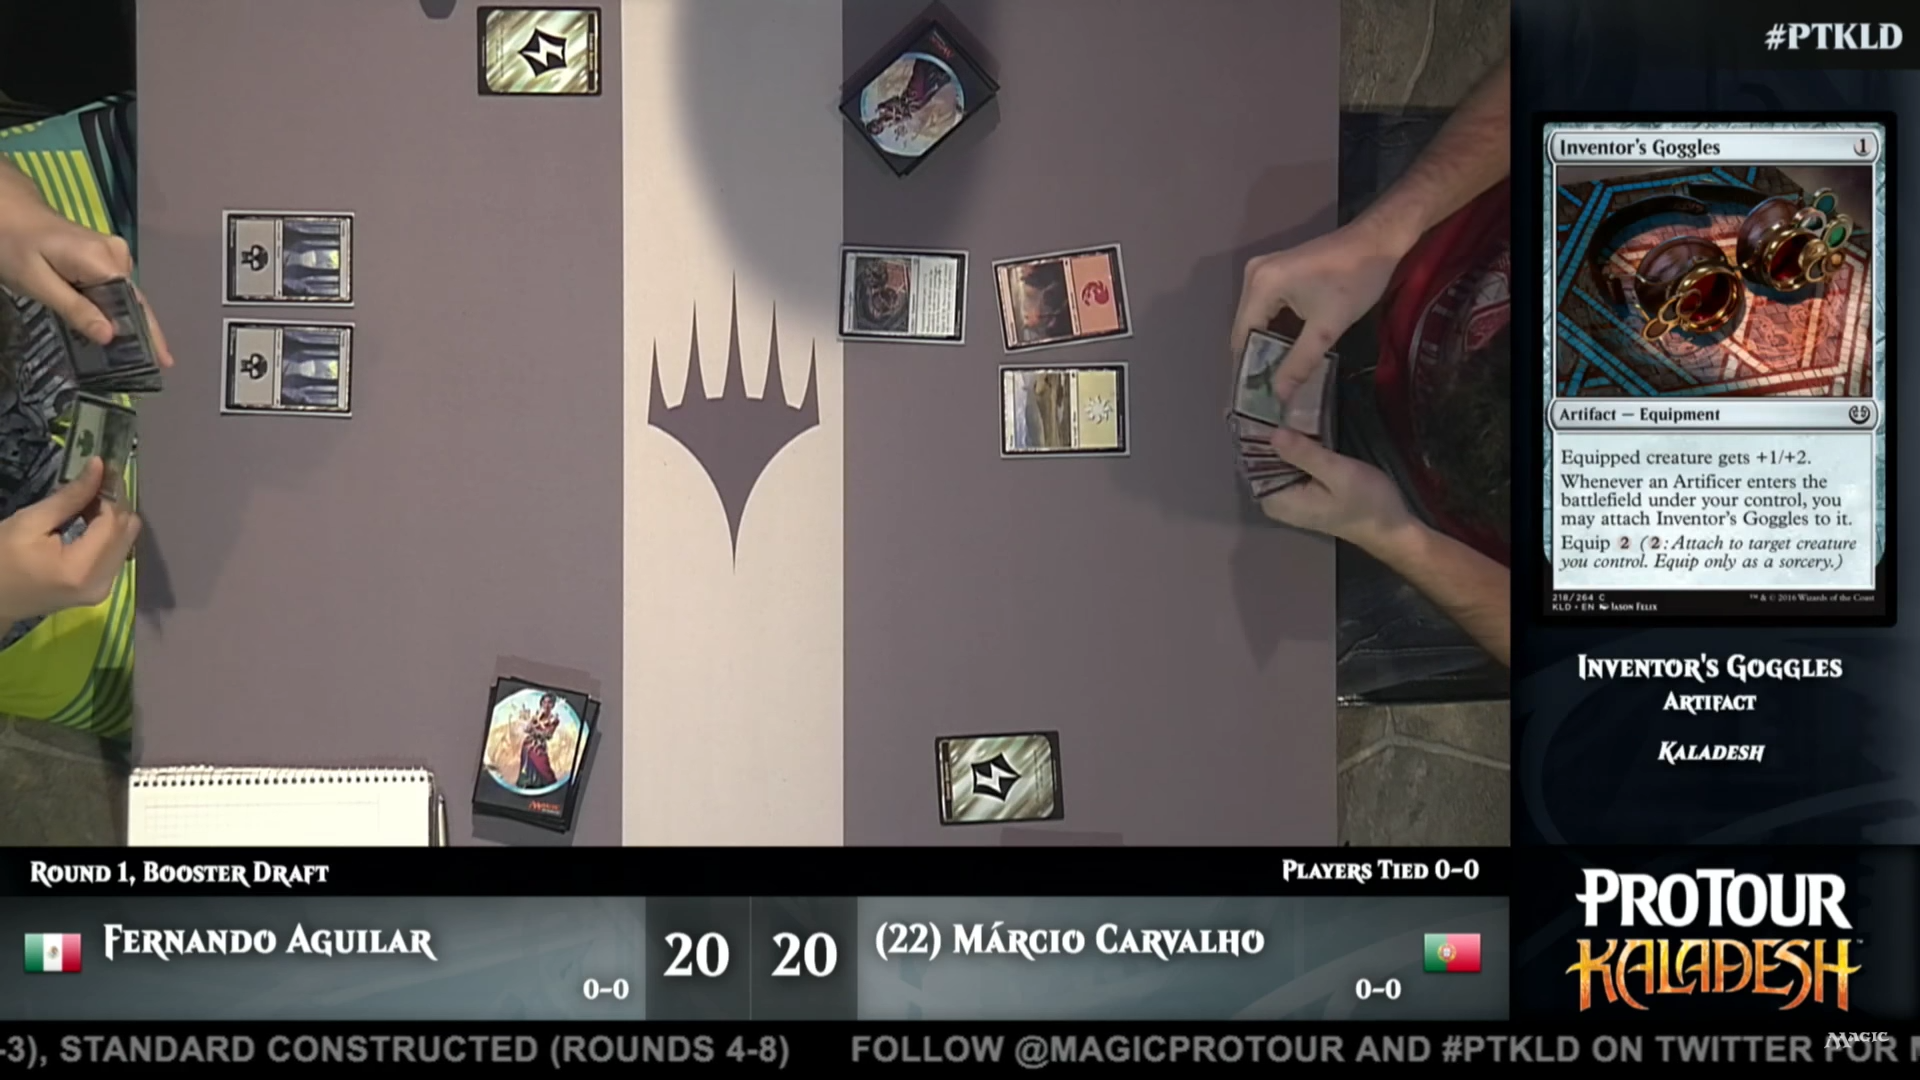
\includegraphics[scale=0.1]{bilder/findCardsSample.png}
    	\caption{Ein Bild aus den Videobildern. Der größte Bereich ist die Aufnahme des Spielbereiches. Rechts daneben befinden sich Informationen zu dem laufenden Turnier. Unterhalb der Spielaufnahme sind Informationen zu den Spielern eingeblendet. }
\label{fig:findCardsSample}
\end{figure}

\subsubsection{Vorverarbeitung}

Bevor in dem Videobild nach Karten gesucht wird, wird das Bild erstmal vorverarbeitet. 
Das Videobild enthält, neben der Aufnahme des Spielbereiches, noch weitere Bereiche mit Informationen für den Zuschauer (siehe Abbildung \ref{fig:findCardsSample}). Um die Karten zu finden, ist nur die Kameraaufnahme des Spielbereiches interessant.
Um nur diesen Bereich zu betrachten, wird das Bild entsprechend zugeschnittten. Das so enstehende Bild (siehe Abbildung \ref{fig:findCardsPreCut}) hat nur noch eine Größe von $1200 \times 845$ Pixeln.


\begin{figure}[h]
    \centering
		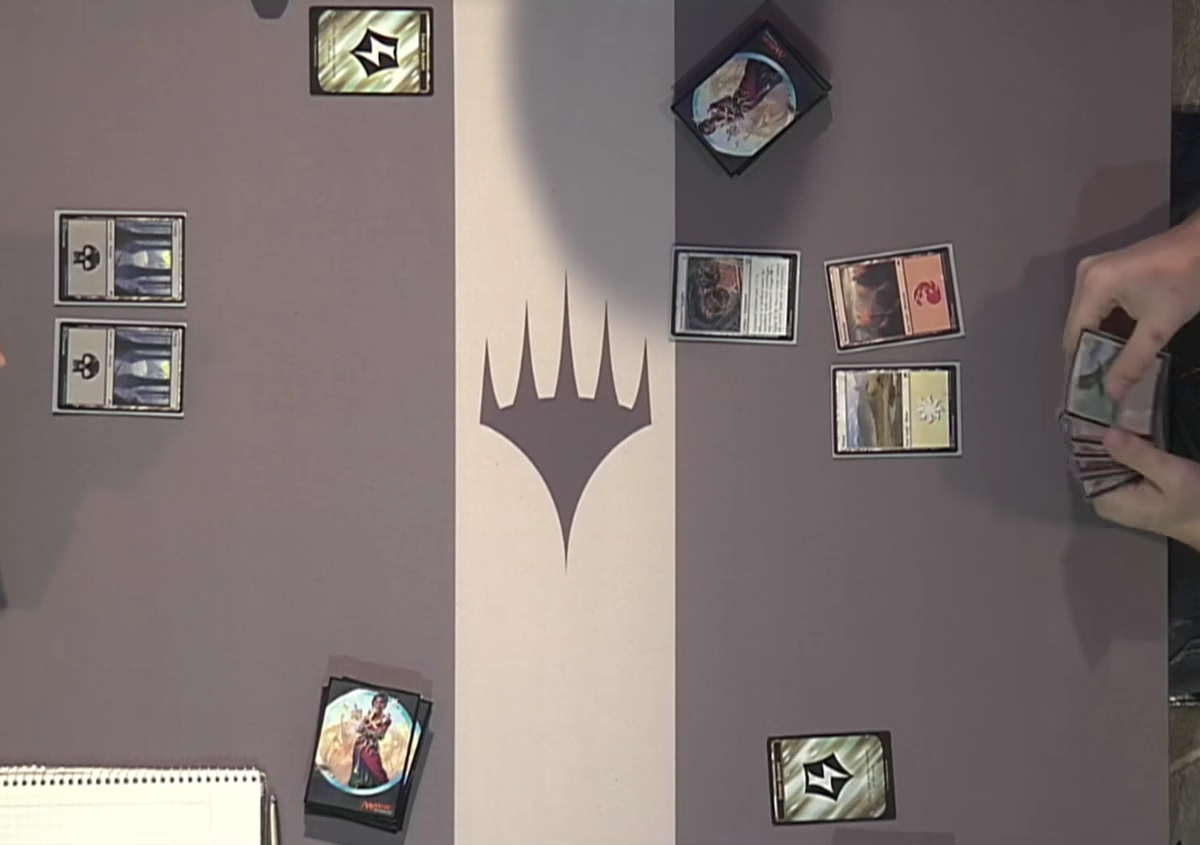
\includegraphics[scale=0.2]{bilder/findCardsPreCut.png}
    	\caption{Das zugeschnittene Bild, sodass nur noch der Spielbereich zu sehen ist.}
\label{fig:findCardsPreCut}
\end{figure}

Damit die Karten in einem späteren Schritt lokalisiert werden könnnen, sollen die Ränder der Karten sichtbar gemacht werden. Dabei kann genutzt werden, dass alle Karten einen schwarzen Rand besitzen.
Das Bild wird zuerst in ein Graubild überführt. In einem Graubild haben schwarze Punkte eine geringe Intensität. Auf diesem Graubild werden alle Pixel, deren Intensität unter einem Schwellwert $t$ liegen, auf den Wert 255 (weiß) gesetzt. Alle Pixel, deren Intensität über dem Schwellwert liegen, werden auf den Wert 0 (schwarz) gesetzt. Das Ergebnis für das Beispielbild kann in Abbildung \ref{fig:findCardsPre} gesehen werden. 
Der Schwellwert wurde experimentell auf $t = 75$ festgelegt.
\begin{figure}[h]
    \centering
		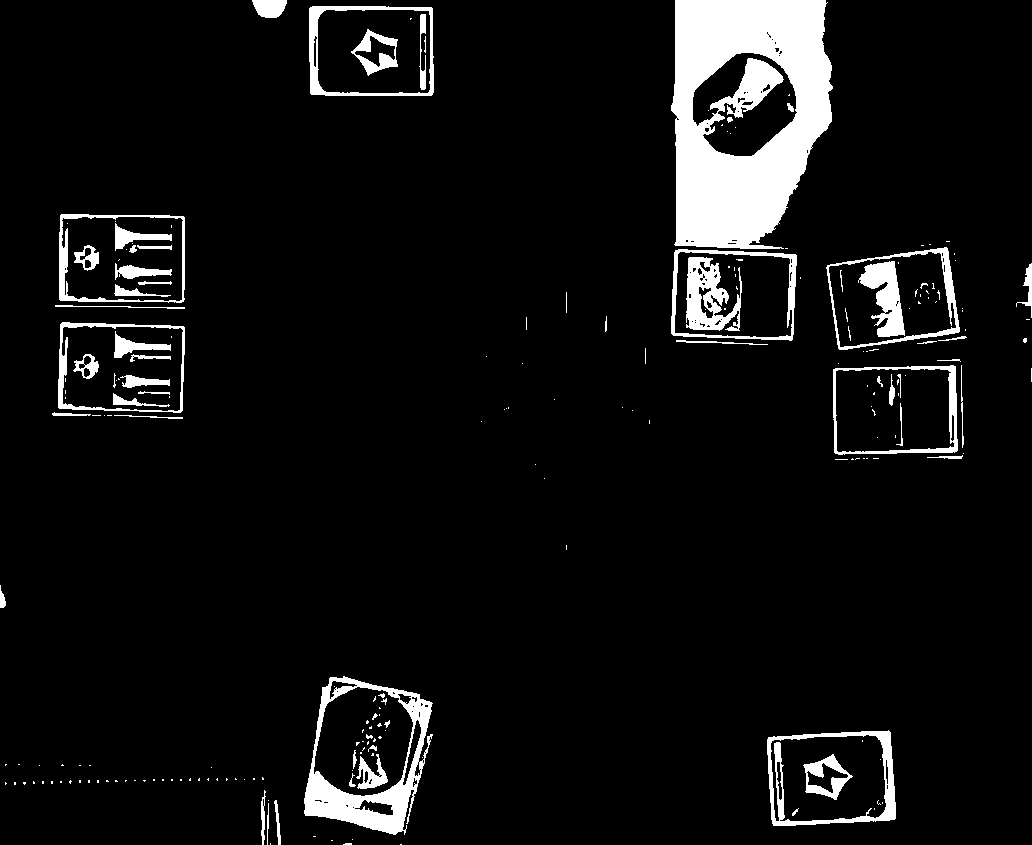
\includegraphics[scale=0.2]{bilder/findCardsPre.png}
    	\caption{Das vorverarbeitete Bild. Die schwarzen Ränder der Karten sind klar erkennbar.}
\label{fig:findCardsPre}
\end{figure}

\subsubsection{Konturerkennung}

Nachdem in der Vorverarbeitung die Ränder der Karten hervorgehoben wurden, sollen nun Konturen erkannt werden, die einer Karte entsprechen.
Zur Konturerkennung wird das von Satoshi Suzuki und Keiichi Abe in ''Topological Structural Analysis of Digitized Binary
Images by Border Following '' \footnote{\cite{journals/cvgip/SuzukiA85}} vorgestellte Verfahren genutzt.

Das Verfahren liefert für jede gefundene Kontur eine Liste an miteinander verbundenen Randpunkten dieser Kontur. Um besser mit der Kontur umgehen zu können, soll die große Liste an Randpunkten reduziert werden. 
Hierfür wird die Kontur mit dem Douglas-Peucker-Algorithmus (siehe \ref{sec:douglas}) approximiert.


\begin{figure}[h]
    \centering
		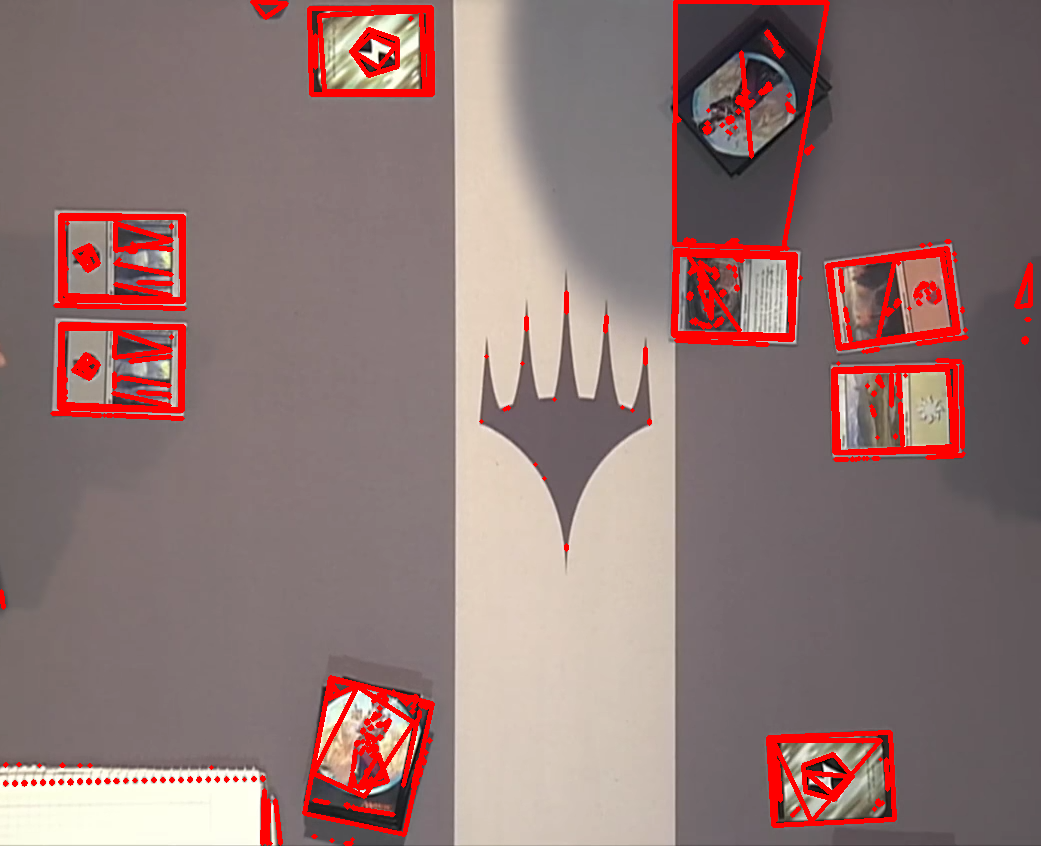
\includegraphics[scale=0.2]{bilder/findCardsContour.png}
    	\caption{Die im vorverarbeiteten Bild gefundenen Konturen sind jeweils rot umrandet.}
\label{fig:findCardsContour}
\end{figure}

Die approximierten Konturen sind in Abbildung \ref{fig:findCardsContour} zu sehen. Ein großer Teil der gefundenen Konturen sind keine Karten. Aus allen gefundenen Konturen sollen die herausgefiltert werden, die keine Karten sind.
Eine Kontur, die zu einer Karte gehört, besteht nach der Approximation nur noch aus vier Randpunkten. Zudem liegt die Größe der Fläche, die diese Kontur einschließt, in einer gewissen Spanne, da alle Karten gleich groß sind.
Aus allen gefunden Konturen werden die gefiltert, die nicht aus vier Punkten bestehen und deren eingeschlossene Fläche kleiner als 5000 und größer als 15000 Pixel ist. Die Grenzen für die Flächen wurden experimentell bestimmt.


Die übrig bleibenden Konturen sind in Abbildung \ref{fig:findCardsFinal} dargestellt.
Die Bildausschnitte in diesen Konturen dienen später als Eingabe für den Klassifikator.

\begin{figure}[h]
    \centering
		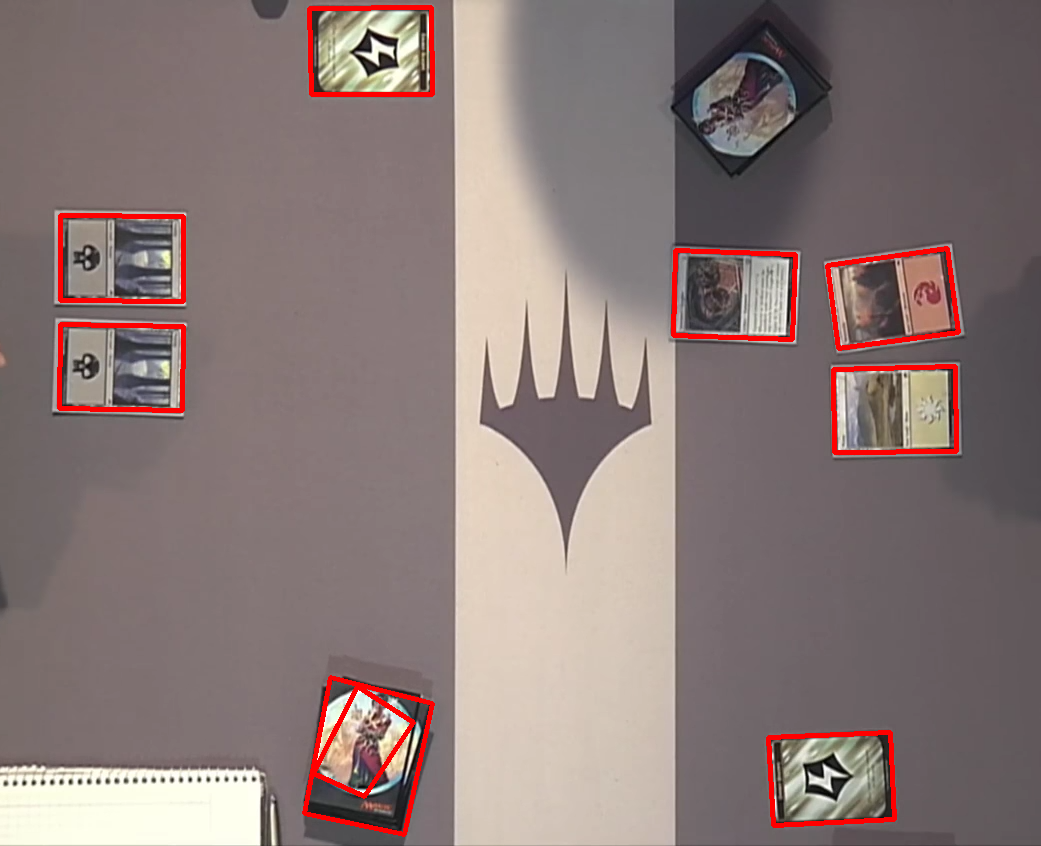
\includegraphics[scale=0.2]{bilder/findCardsfinal.png}
    	\caption{Alle Konturen, die nicht gefiltert wurden.}
\label{fig:findCardsFinal}
\end{figure}


\subsection{Erweiterung des Trainingsdatensatzes}

Mit dem in \ref{sec:kartenFinden} gezeigten Verfahren zur Lokalisierung von Karten und dem Klassifikator soll der Trainingsdatensatz erweitert werden.

\subsubsection{Idee}

Mit einer Kombination aus Lokalisierung und Klassifikation können Karten automatisch aus einem Video herausgeschnitten und klassifiziert werden.
Das Video wird durchlaufen und in regelmäßigen Abständen wird in dem Videobild nach Karten gesucht. Sobald die Karten lokalisiert wurden, werden diese automatisiert, anhand der gefundenen rechteckigen Kontur, ausgeschnitten. 
Diese Bildausschnitte werden mit dem in \ref{sec:klassifikator} beschriebenen Klassifikator klassifiziert. Es soll vermieden werden, dass falsch klassifizierte Karten in den erweiterten Trainingsdatensatz aufgenommen werden. Um dies zu verhindern, wird eine so klassifizierte Karte nur in den erweiterten Trainingsdatensatz aufgenommen, wenn ihr Softmax Wert über einer bestimmten Schwelle liegt.

Als Trainingsvideos werden die Videos in der YouTube Playlist \url{https://www.youtube.com/playlist?list=PLyUK7d88voIirGp0IbtppzOAuMVC4ZVcW} genutzt.

\subsubsection{Implementierung}

Jedes der Videos wird einmal komplett durchlaufen. Da zwischen aufeinanderfolgenden Videobildern kein großer Unterschied besteht, wird nicht jedes einzelne Bild betrachtet.
Es wird nur jedes 180te Videobild betrachtet. Da die Videos 30 Bilder pro Sekunde haben, entspricht das einer Wartezeit von 6 Sekunden.
Bei jedem betrachtetem Bild werden zuerst Bildausschnitte mit dem in \ref{sec:kartenFinden} beschriebenen Verfahren gefunden. 

Die gefundenen Bildausschnitte werden mit dem Klassifikator klassifiziert.
Der Klassifikator wird hierbei mit ORB verwendet. Die Wahl für ORB ist daduruch begründet, dass es das schnellste Verfahren ist und eine gute Erkennungsrate hat (siehe \ref{sec:auswertung}).

Um falsche Klassifikationen nicht mit in den erweiterten Testdatensatz aufzunehmen, wird der Softmax Wert für die Klassifikation betrachtet. Liegt dieser über einer Schwelle $t = 0.8$, so wird die ausgeschnittene Karte als Bild mit der gefundenen Klasse gespeichert. Der Wert von $t = 0.8$ wird gewählt, da in Abbildung \ref{fig:hist} beobachtet wurde, dass fast alle Softmax Werte richtig klassifizierter Karten über 80\% liegen. So werden fast alle richtig klassifizierten Karten über dem Schwelllwert liegen und jede falsch klassifizierte unter ihm.
